\documentclass[main.tex]{subfiles} 
\begin{document}

\section*{Analyse}
\label{sec:2}

Hvordan ble undervisningen lagt opp for å skape god begrepsforståelse i naturfagstimen, og hvordan 
bidro gruppesamtalene til dette? For å svare på dette, la oss se nærmere på hele 
undervisningssekvensen.

\subsection*{Aktivering av forkunnskaper}
Ved oppstarten av timen ble dialog initiert av læreren. Helklassesamtalene hadde preg av
IRE/F metoden (\citeNP{klet13}), dvs. lærer tar initiativ(I), elev responderer(R) og responsen blir 
evaluert(E) og/eller kommentert(F). Til denne sekvensen rekker elevene opp hånda for å respondere. 
Det viser seg at det er noen få elever som er villig til å svare, oftest de flinke elevene. Dette 
er uheldig siden flerparten av elevene er ikke aktive. Dermed får de ikke brukt denne sekvensen som
en anledning til å trene i å bruke naturfaglige begreper, som igjen bidrar til å øke deres forståelse
(\citeNP[s. 176]{klet13}).
\newline
\newline
Bruken av revoicing til å gjenta og forsterke elevenes forslag og begrepsbruk ble ikke brukt 
tilstrekkelig gjennom denne sekvensen. Ifølge Klette, viser fravær av slike eksplisitte 
innramminger fra lærerens side at eleven blir sittende med et uklart kunnskapsinnhold og i 
verste fall feil begrepsforståelse, \citeA[s. ~175-176]{klet13}. For å kunne bruke revoicing 
mest mulig effektivt, må læreren raskt kunne bestemme om elevens repons har validitet 
og om det er relevant. Gjennom prasiserfaringen har revoicing vært vanskelig å utføre. Ved å 
forutse elevsvar før elever i klassen blir initiert, kan misforståelser som ofte oppstår bli 
redegjort av læreren, og respons som ofte opptrer kan tas stilling til. Dette krever derimot 
en god del erfaring fra læreren sin side. I \citeA[s. ~401]{batp08} klassifiseres dette som 
``knowledge of content and students, (KCS)''. Over tid vil en lærer danne omfattende KCS og
dette kan dermed bidra til å øke kvaliteten på helklassesamtalene. 

\subsection*{Innføring av nytt tema - under konstruksjon}
\citeA[s. 77]{solv92} skriver at forståelse er aktivert kunnskap. Det vil si hver gang vi utsettes 
for en utfordring blir vårt eget \emph{kunnskapsreservoar} tappet og vi aktiverer vår kunnskap. 
Elevenes kunnskaper utgjør en av forutsetningene for de nye kunnskapene vi tilfører dem. Disse 
kunnskapene, sammen med elevenes erfaringer, utgjør det eleven kan møte nye utfordringer med. Dette 
betegnes også som kognitiv struktur og kan deles opp i delstrukturer. Piaget 
kaller slike delstrukturer for skjemaer (\citeNP[s. 78]{solv92}). En elev har for eksempel ett skjema 
for encellede organismer og ett for flercellede organismer. Det som er karakterisktisk for slike 
skjemaer er at de kan operere sammen. Hvis eleven behersker begge disse begrepene, kan eleven danne 
koblingen mellom disse skjemaene og dermed danne flere assosiasjoner til levende oraganismer. 
De kan da ha muligheten til å danne forbindelsen mellom komplekse organismer som mennesker til enkle 
organismer som bakterier. I dette tilfellet blir store spørsmål som hvor og hvordan ble liv utviklet 
på jorden bli sett i perspektiv av biologisk mangfold. På denne måten konstrueres ny kunnskap ved hjelp 
av den kunnskapen eleven allerede har.
\newline
\newline
Hver elev vil ha sine skjemaer til å møte undervisning med. Innledning til temaet encellede organismer ble innført
\newline
\newline
Fra figur \ref{fig:odeg10} kan vi se at i en vanlig naturfagstime brukes mye tid på å formidle 
nytt fagstoff, og det er lite konsolideringssituasjoner. 


\begin{figure}[h!]
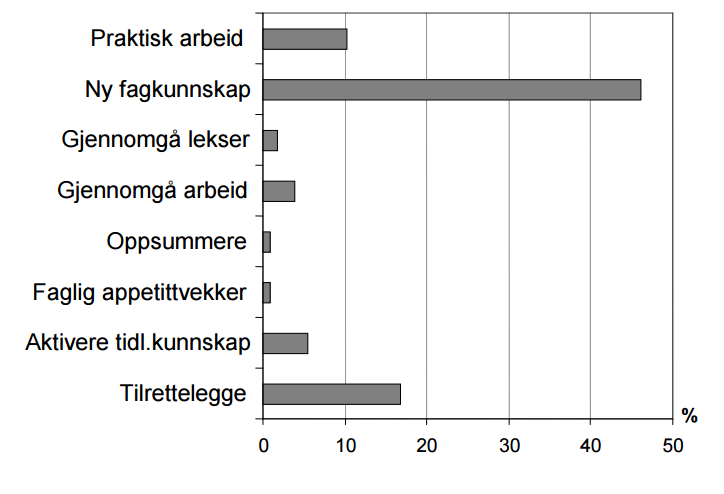
\includegraphics[scale = 0.6]{../figures/undervisnings_aktivitet.png}
\caption{Oversikt over naturfaglærernes undervisningstilbud til elevene fra PISA+ studie. Kilde: 
\protect\citeA{odeg10}.}
\label{fig:odeg10}
\end{figure}

\subsection*{Gruppe samtaler - under konstruksjon}
Den sosiokulturelle teorien har utgangspunkt (\citeNP[s. 13]{meli07}; \citeNP[s. 123]{bta98}; 
\citeNP[s. 87]{rogs13}; \citeNP[s. 299]{sjob04}; \citeNP[s. 62]{knai11}) i Lev Vygotsky sine 
perspektiver på læring og utvikling. Blant disse perspektiver var Vygotskys syn på at barns 
intellektuelle utvikling er formet utfra tilegnelse av språk, fordi språk muliggjør dialog 
mellom mennesker (\citeNP[s. 5]{meli07}). Dette har senere fått empirisk støtte, og har 
implikasjoner for utdanningspraksis(\citeNP[s. 83]{meli07}).
\newline
\newline
I helklassesamtalen ved starten av timen var det et fåtall elever som var aktive i lærer initiert 
diaglog. Dette var uheldig siden elevenes styrker og svakheter ble ikke tilstrekkelig avdekket. 
Gruppesamtalene viste seg å være en god plattform for å avdekke hull og svakheter i elevenes 
begrepsbruk. I den forbindelse ble tokolonnenotatet tatt i bruk (se vedlegg: 
\ref{sec:tokolonnenotat}).
\newline
\newline
I tokolonnenotatøvelsen viste noen grupper akkumulative tendenser. Det vil si at elevene 
var villig til å akseptere hverandres bidrag uten å stille kritiske spørsmål og fremsette
alternative eller utfyllende forklaringer. Noen elever som jobbet i en gruppe, arbeidet så og si
selvstendig ved å føre rett inn i sine egene utdelte kopier av tokolonnenotatet, et sluttresult som 
ikke var basert på et felles grunnlag. Dermed fikk de en annen type utbytte fra gruppearbeidet
enn det som var tiltenkt; ``groupsense or feeling of a shared endeavour'' (\citeNP[s. 25]{meli07}). 
Med andre ord ble det et samarbeid og ikke en kollaborasjon, som \citeA{meli07} respektivt kaller 
\emph{interacting vs. interthinking}. Gruppen endte opp med et felles produkt, men det var ikke 
basert på en kollaborasjon mellom elevene. Målet med et samarbeid er å ende opp med en sluttprodukt. 
I motsetning er en kollaborasjon der individer frembringer egene ideer til gruppen, og hver ide
blir da vurdert og diskutert felles i gruppen: enten blir den akseptert eller så forkastes den.
\newline
\newline
En viktig del av den sosiale utprøvingen av ideer og begreper innebærer å sammenlikne egne 
forestillinger med andres forestillinger i tillegg til naturvitenskapens forklaringer 
(\citeNP{odeg10}; \citeNP{dals94}). Bruken av tokolonnenotatet i første timen 
\newline
\newline
Når elevene deretter ble fordelt i andre grupper og prøvde å presentere begrepene, viste noen elever 
svak forståelse. I blant ble begrepene fremstilt overfladisk, og for noen elever ble deres svakheter 
om temaene avdekket. Noen elever til en viss grad misbrukte øvelsen ved å avskrive notatene til sine 
medelever. Til deres forsvar kan det sies at instruksene som ble formidlet var ikke tydelige nok. 
Uansett ble denne oppførsel irettesatt og klarere instrukser ble formidlet.
\newline
\newline
Den \emph{nærmeste utviklingssonen} beskriver en sone som ligger i mellom et barns kognitive 
ferdigheter, dvs. hva de kan oppnå selvstendig uten hjelp, og potensielle utviklingen, dvs. 
hva et barn kan få til eller forstå gjennom enten veiledning eller kollaborasjon 
(\citeNP[s. 14]{meli07}; \citeNP[s. 125]{bta98}; \citeNP[s. 75]{rogs13}). ``Scaffolding'' 
eller stillasbygging (\citeNP{bta98}; \citeNP[s. 71]{math15})
\newline
\newline
Gode fagsentrerte samtaler mellom elever (eller faglige samtaler med lærer) hvor elever bruker egne 
erfaringer og språket for å oppnå faglig forståelse hjelper til å skape bro mellom praksis og teori 
(\citeNP{odeg10}).
\newline
\newline
Evnen til abstrahering henger ifølge Vygotsky (\citeNP[s. 127]{bta98}) med begrepsundervisning, som en
form for vitenskapeliggjøring av hverdagsbegreper. Hvis elever ikke har god begrepsforståelse
kan de ende opp med å bruke naturvitenskapelige begreper i feil kontekst og danne feil 
forbindelser med begrepene. Dette avhenger av deres forkunnskaper. Ausubels kognitive bruer 
(\citeNP[s. 71]{math15}), hans teori om begrepslæring på høyere nivå og hvordan læreren best kan 
legge til rette for slik læring og bruk av begrepene, handler om å danne forbindelser mellom 
undervisningsmateriell og relevante ideer i elevenes kognitive struktur.

\end{document}